\iffalse
\documentclass[journal,10pt,twocolumn]{article}
\usepackage{graphicx}
\usepackage[margin=0.5in]{geometry}
\usepackage[cmex10]{amsmath}
\usepackage{array}
\usepackage{booktabs}
\title{\textbf{Line Assignment}}
\author{Mohamed Hamdan}
\date{September 2022}

\providecommand{\norm}[1]{\left\lVert#1\right\rVert}
\providecommand{\abs}[1]{\left\vert#1\right\vert}
\let\vec\mathbf
\newcommand{\myvec}[1]{\ensuremath{\begin{pmatrix}#1\end{pmatrix}}}
\newcommand{\mydet}[1]{\ensuremath{\begin{vmatrix}#1\end{vmatrix}}}
\providecommand{\brak}[1]{\ensuremath{\left(#1\right)}}

\begin{document}

\maketitle
\fi
 $ABC$ is a triangle right angled at $\vec{C}$. A line through the mid-point $\vec{M}$ of hypotenuse $AB$ and parallel to $BC$ intersects $AC$ at $D$ (see Fig.  
		\ref{fig:9/8/2/7}).
Show that
\begin{enumerate}
	\item $D$ is the mid-point of $AC$
	\item $MD \perp AC$
	\item $CM = MA = \frac{1}{2}AB$
\end{enumerate}
	\begin{figure}[!h]
		\centering
 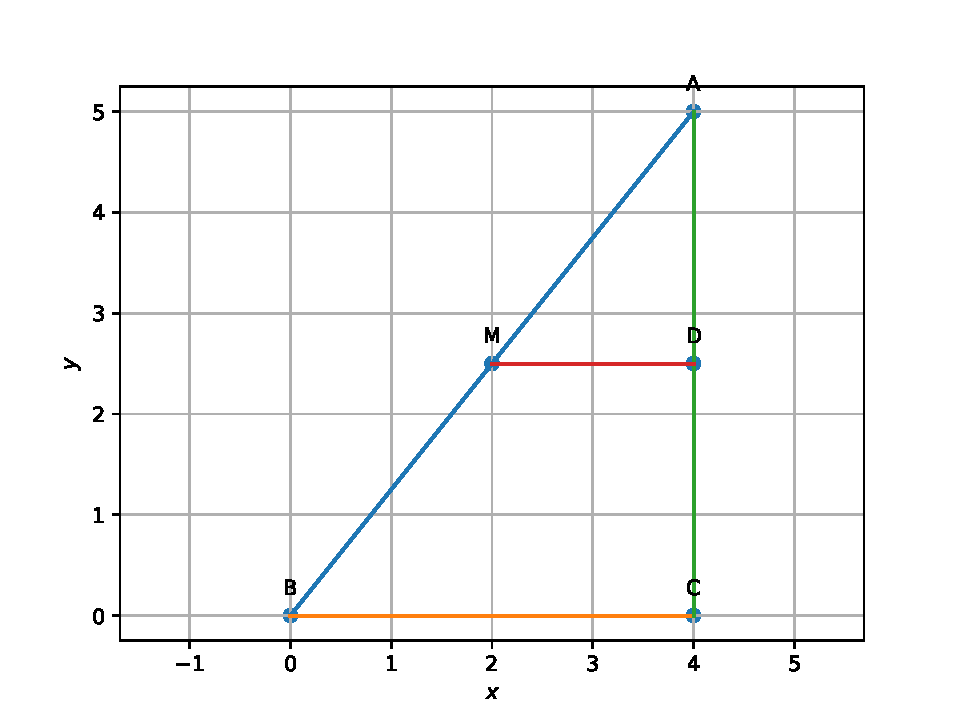
\includegraphics[width=\columnwidth]{chapters/9/8/2/7/figs/fig1.pdf}
		\caption{}
		\label{fig:9/8/2/7}
  	\end{figure}
	\solution 
	\begin{enumerate}
\item Trivial from  Appendix
		\label{prop:9/8/2/7}
	  \ref{prop:two-tri-bpt-conv}.
  \item 
Since $ABC$ is right angled at $C$,
\begin{equation}
	(\vec{C}-\vec{A})^{\top}(\vec{C}-\vec{B}) = 0	
\label{eq-3}
\end{equation}
Given that $MD$ is parallel to $BC$, so
\begin{equation}
	(\vec{C}-\vec{B}) = \lambda(\vec{M}-\vec{D})
\label{eq-4}
\end{equation}
Substituting (\ref{eq-4}) in (\ref{eq-3}) and dividing by $\lambda$, we get
\begin{equation}
	(\vec{C}-\vec{A})^{\top}(\vec{M}-\vec{D}) = 0	
\label{eq-5}
\end{equation}
From (\ref{eq-5}) it can be concluded that $MD \perp AC$.
\item Since
\begin{align}
	\norm{\vec{C}-\vec{M}}^2-\norm{\vec{A}-\vec{M}}^2 &= 	
	\norm{\vec{C}}^2-\norm{\vec{A}}^2-2\brak{\vec{C}-\vec{A}}^{\top}\vec{M} 
	\\
	&=\brak{\vec{C}-\vec{A}}^{\top}\brak{\vec{C}+\vec{A}-2\vec{M}} 
	\\
	&=\brak{\vec{C}-\vec{A}}^{\top}\brak{\vec{C}-\vec{B}} = \vec{0} 
\label{eq:9/8/2/7/sides}
\end{align}
upon substituting from 
Property		\ref{prop:9/8/2/7}
and 
\eqref{eq-3}.  Thus, $CM = AM$.

	\end{enumerate}

\iffalse
\section*{Solution}

\subsection*{Part 1}
Given MN is $\parallel$ to BC, hence\\
\begin{equation}
\frac{AD}{DC} = \frac{AM}{MB}
\label{eq-1}
\end{equation}
Since M is the mid-point of AB, $\frac{AM}{MB} = 1$. Substituting in (\ref{eq-1}), we get\\
\begin{equation}
AD = DC
\label{eq-2}
\end{equation}
Therefore, D is the midpoint of AC.

\subsection*{Part 2}
\subsection*{Part 3}
Let
\begin{eqnarray}
	\boldsymbol{M-D} = \boldsymbol{p}\\
	\boldsymbol{C-D} = \boldsymbol{q}\\
	\boldsymbol{A-D} = \boldsymbol{r}
\end{eqnarray}
Then vectors along CM and AM can be written as
\begin{eqnarray}
	\boldsymbol{C-M} = \boldsymbol{q-p}\\
	\boldsymbol{A-M} = \boldsymbol{r-p}
\end{eqnarray}
The magnitudes of CM and AM are therefore
\begin{eqnarray}
	||\boldsymbol{C-M}|| = ||\boldsymbol{q-p}|| = (\boldsymbol{q-p})^T(\boldsymbol{q-p})\\
	||\boldsymbol{A-M}|| = ||\boldsymbol{r-p}|| = (\boldsymbol{r-p})^T(\boldsymbol{r-p})\\
\end{eqnarray}
Upon expanding the vector products, the terms $\boldsymbol{q}^T\boldsymbol{p}$ and $\boldsymbol{r}^T\boldsymbol{p}$ evaluate to 0 (from eq.\ref{eq-5}). From eq.\ref{eq-2}, $$||\boldsymbol{q}|| = ||\boldsymbol{r}||$$. Therefore,
\begin{equation}
||\boldsymbol{C-M}|| = ||\boldsymbol{q}|| + ||\boldsymbol{p}||\\
\label{eq-4-}
\end{equation}
\begin{equation}
||\boldsymbol{A-M}|| = ||\boldsymbol{r}|| + ||\boldsymbol{p}|| = ||\boldsymbol{q}|| + ||\boldsymbol{p}||
\label{eq-3-}
\end{equation}
Equating (\ref{eq-4-}) and (\ref{eq-3-}), we get
\begin{equation}
AM = CM
\label{eq-2-}
\end{equation}
Since given that M is midpoint of AB, 
\begin{equation}
AM = \frac{1}{2}AB
\label{eq-1-}
\end{equation}
Equating (\ref{eq-2-}) and (\ref{eq-1-}), the result is proved.

\section*{Construction}
The input parameters are the lengths a and c.\\
{
\setlength\extrarowheight{2pt}
\begin{tabular}{|c|c|c|}
	\hline
	\textbf{Symbol}&\textbf{Value}&\textbf{Description}\\
	\hline
	a&4&BC\\
	\hline
	c&5&AC\\
	\hline
	k&1&$\frac{AM}{MB} = \frac{AD}{DC}$\\
	\hline
	$\theta$&arctan($\frac{c}{a}$)&$\angle$B\\
	\hline
	A&$\sqrt{a^2+c^2}%
	\begin{pmatrix}
		cos\theta\\
		sin\theta\\
	\end{pmatrix}$%
	&Point A\\
	\hline
\end{tabular}
}

\section*{Proofs}
Let the vertices of the triangle be $\vec{A}, \vec{B}, \vec{C}$ such that  
		\begin{align}
			\vec{B} =\vec{0} 
		\end{align}
		and $\vec{A}, \vec{C}$ are known. Let $\vec{P}$ be a known point on $AB$ such that $PQ$ is parallel to $BC$.  Let 
		\begin{align}
			\vec{P} &= \lambda \brak{\vec{A} -\vec{B} }
			\label{eq:cbse-2020-10-bpty}
			\\
			&=\lambda 
			 \vec{A} 
			\label{eq:cbse-2020-10-bpt}
			\\
			\text{and , } \frac{\norm{\vec{P} 
			}}{\norm{\vec{A}} } &= \frac{BP}{AB}= \abs{\lambda}
			\label{eq:cbse-2020-10-bpt-pa}
		\end{align}
		Since 
		\begin{align}
			PQ &\parallel BC,
			\\
			\vec{Q} &= P + \mu \vec{B-C}
			\\
			&= \lambda \vec{A} - \mu \vec{C}
			\label{eq:cbse-2020-10-bpt-q1}
		\end{align}
		using the equation of the line $PQ$  and substituting from 
			\eqref{eq:cbse-2020-10-bpt}
			Also, since $\vec{Q}$  lies on the line $AC$, 
		\begin{align}
			\vec{Q} &= \vec{A} + k \brak{\vec{A}-\vec{C}}
			\\
			&= \brak{1 + k}\vec{A} - k \vec{C}
			\label{eq:cbse-2020-10-bpt-q2}
			\\
			\text{and }\frac{\norm{{\vec{A}-\vec{Q}}}}{\norm{{\vec{A}-\vec{C}}}} &= \frac{AQ}{AC}= \abs{k}
			\label{eq:cbse-2020-10-bpt-q2k}
		\end{align}
			From \eqref{eq:cbse-2020-10-bpt-q1} and 
			\eqref{eq:cbse-2020-10-bpt-q2}
		\begin{align}
			\lambda \vec{A} - \mu \vec{C}	= 
			 \brak{1 + k}\vec{A} - k \vec{C}&
			\\
			\implies 
			\brak{1 + k+\lambda }\vec{A} \brak{k - \mu}  \vec{C}	&=  0
			\\
			\implies k = \mu, \lambda = -1 - \mu 
			\\
			\text{or, } \abs{\lambda } = 1 + k
			\label{eq:cbse-2020-10-bpt-q2-lk}
		\end{align}
		From 
			\eqref{eq:cbse-2020-10-bpt-pa},  
			\eqref{eq:cbse-2020-10-bpt-q2k} and
			\eqref{eq:cbse-2020-10-bpt-q2-lk},
			\begin{align}
				\frac{AQ}{AC} = \frac{AP}{AB}
			\end{align}
\end{document}
\fi
